%%
% BIThesis 研究生学位论文模板 The BIThesis Template for Graduate Thesis
% This file has no copyright assigned and is placed in the Public Domain.
%%

\chapter{面向多智能体系统的消息压缩框架}

\section{研究内容}

在这一章节中，我们将详细阐述如何将通信优化嵌入多智能体系统任务执行流程，并解析各个功能模块的具体设计。

\subsection{研究方案概述}

在这一章节中，我们将描述当前多智能体执行的流程，并给出消息压缩框架的初步设计。

\subsubsection{多智能体系统任务执行流程}

多智能体系统通过角色分工与协作推理来完成目标。如图\ref{fig:mas_workflow}所示，其标准任务执行流程主要包含以下四个核心环节：

\begin{enumerate}[
    topsep=0pt,
    itemsep=0pt,
    parsep=0pt,
    partopsep=0pt,
    leftmargin=0em,
    itemindent=2em,
    label=\arabic*.
]
    \item \textbf{任务输入：}接收并标准化外部任务，为智能体构建结构化的上下文环境。
    \item \textbf{协作推理：}依托预设的通信拓扑，各智能体结合自身角色与前驱节点的历史信息进行多轮次推理，并持续传递中间结果。
    \item \textbf{结果聚合：}采用投票或共识决策机制，对各智能体的候选答案进行汇总，输出最终可靠结果。
    \item \textbf{性能评测：}系统性评估模型在任务准确率及通信成本（如词元消耗、推理延迟）上的综合表现。
\end{enumerate}

\begin{figure}[htbp]
    \centering
    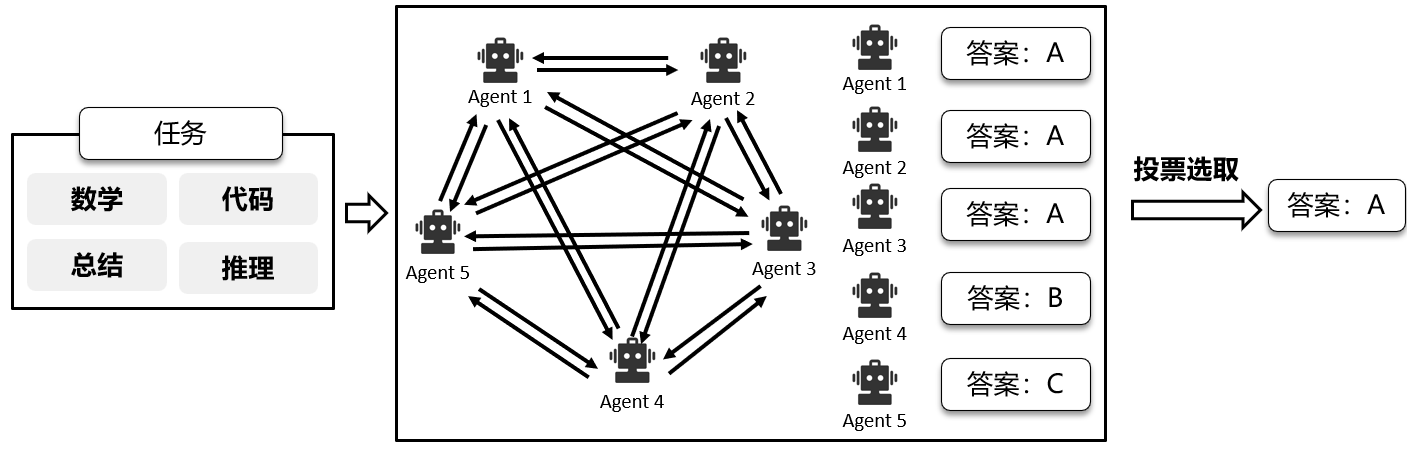
\includegraphics[width=0.85\linewidth]{image/第二章/图 2‑1 多智能体系统标准任务执行流程示意图.png}
    \caption{多智能体系统标准任务执行流程示意图}
    \label{fig:mas_workflow}
\end{figure}

\subsubsection{消息压缩框架执行流程}

为解决多智能体协作中的信息冗余问题，本课题在智能体与智能体之间的通信中引入了\textbf{消息压缩框架}。该框架从角色、节点和时序三个维度对通信内容进行压缩。

具体执行流程包含以下三个核心步骤：

\begin{enumerate}[
    topsep=0pt,
    itemsep=0pt,
    parsep=0pt,
    partopsep=0pt,
    leftmargin=0em,
    itemindent=2em,
    label=\arabic*.
]
    \item \textbf{角色感知压缩：}针对接收方信息需求的不对称性，根据下游角色的具体职责，过滤前驱智能体消息中的无关推理内容，从而使下游智能体能够获得与自身任务更相关的信息。
    \item \textbf{节点感知聚合：}针对多个前驱节点可能产生相似推理内容的问题，将不同节点传来的相似推理过程进行去重，避免相同观点在下游智能体上下文中重复出现，从而减少冗余消息传递。
    \item \textbf{分歧感知压缩：}针对多轮对话记录过长的问题，通过提取历史轮次中的共识与分歧内容，压缩上一轮次传递的信息，并保留有效信息供本轮智能体参考。
\end{enumerate}

\begin{figure}[htbp]
    \centering
    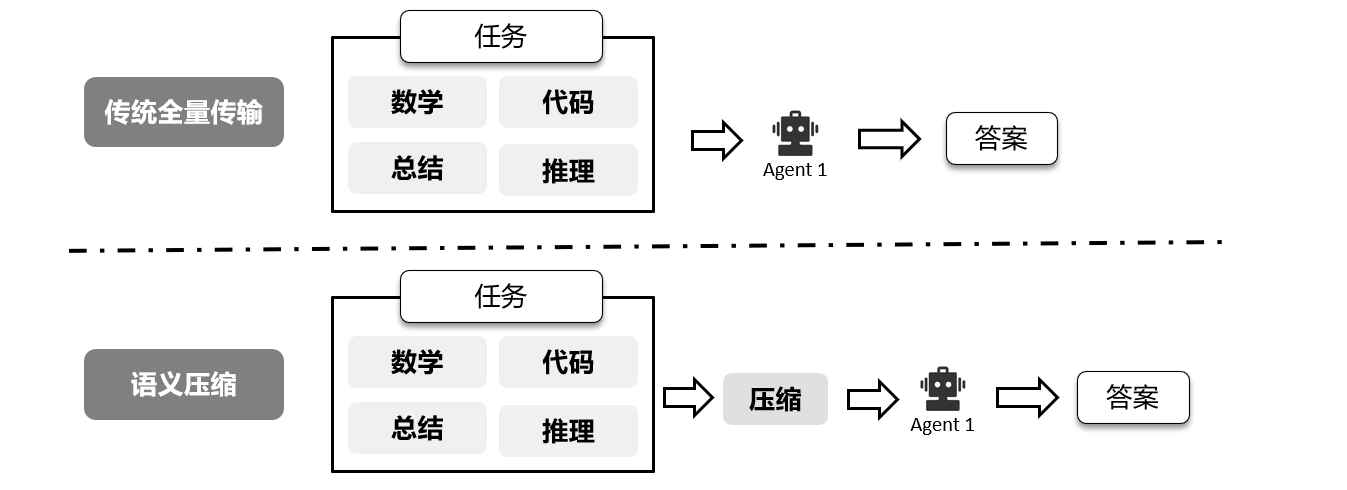
\includegraphics[width=0.85\linewidth]{image/第二章/图2-2 消息压缩框架.png}
    \caption{消息压缩框架}
    \label{fig:message_compression_framework}
\end{figure}


\subsection{功能模块设计}

本节介绍消息压缩框架的三个核心模块：角色感知消息压缩、节点感知消息聚合和时序答案一致性摘要。三者分别处理多智能体通信中的三类冗余：第一类是发送方推理内容与接收方角色无关，第二类是多个前驱智能体给出了相似推理，第三类是跨轮历史持续累积导致上下文过长。为避免符号堆叠，本文仅保留必要定义，并重点说明各模块的输入、处理逻辑和输出结果。

设多智能体系统的通信图为$G=(V,E)$。在第$t$轮中，发送方智能体$u$传递给接收方智能体$v$的消息表示为
$$
m_{u\rightarrow v}^{(t)}=(r_u^{(t)},a_u^{(t)}),
$$
其中$r_u^{(t)}$表示推理内容，$a_u^{(t)}$表示最终答案。本文的压缩操作主要作用于推理内容$r_u^{(t)}$，原则上不直接改写答案字段，从而避免压缩过程破坏最终判断。

\subsubsection{角色感知压缩模块}

角色感知压缩模块解决的是“消息是否适合当前接收方”的问题。在多智能体系统中，不同智能体承担的职责不同。例如，负责规划的智能体更需要任务拆解和约束信息，负责验证的智能体更关注候选答案、错误风险和反例。如果发送方的完整推理被直接转发给所有下游节点，接收方会同时看到大量与自身职责无关的内容，既增加token成本，也容易稀释真正有用的信息。

该模块的处理流程分为三步。首先，将发送方的推理文本按句子切分，得到若干候选推理片段。其次，将每个句子与接收方角色描述进行语义匹配，匹配分数由文本向量的余弦相似度给出：
$$
\operatorname{sim}(s,d_v)=\cos(\phi(s),\phi(d_v)),
$$
其中$s$表示候选句子，$d_v$表示接收方角色描述，$\phi(\cdot)$表示文本编码函数。最后，系统根据同一条消息内部的相似度分布自动确定保留阈值，只保留与接收方角色更相关的句子；若保留文本仍超过角色预算，则按原始顺序截断到预算范围内。

该模块的输出仍然是一条结构化消息：推理字段被替换为筛选后的短文本，答案字段保持不变。这样做的好处是，接收方能够获得更贴近自身职责的上下文，同时不会因为压缩推理过程而丢失发送方给出的最终答案。

\subsubsection{节点感知聚合模块}

节点感知聚合模块解决的是“多个前驱消息之间是否重复”的问题。对于同一个接收方节点，多个上游智能体可能从不同角度得出相近结论，也可能在推理过程中反复陈述同一事实。如果将这些内容直接拼接，下游节点会接收到大量重复表达，导致上下文变长，但信息增量有限。

该模块会先收集接收方节点所有前驱智能体的压缩后推理句子，并为每个句子保留来源角色标签。随后，系统按照句子出现顺序逐一检查候选内容：若当前句子与已保留句子的语义相似度高于冗余阈值，则认为它提供的信息已经被覆盖，不再重复加入；若相似度低于阈值，则将其作为新的有效信息保留。本文实现中，冗余判定阈值取$0.70$，用于在“去重”和“保留多样观点”之间取得平衡。

聚合后的推理内容由若干带角色标签的句子组成。角色标签的作用是保留信息来源，使下游智能体不仅知道“有哪些观点被保留”，也能知道“这些观点来自哪个角色”。对于多个前驱节点给出的答案，模块采用简单投票生成聚合答案；若出现票数接近或无法明确多数的情况，则保留多个候选答案及其来源，交由后续节点继续判断。

通过该模块，系统不再把多个前驱消息拼接，而是先做跨节点去重和来源标注。这样既能减少重复token，也能提高下游上下文的信息密度。

\subsubsection{分歧感知压缩模块}

分歧感知压缩模块解决的是“跨轮历史如何保留”的问题。多智能体协作通常需要多轮执行，如果每一轮都完整保存所有智能体的推理和答案，历史记忆会快速膨胀。过长的历史不仅增加推理成本，还可能使模型在后续轮次中难以抓住当前最关键的共识和分歧。

该模块在每一轮协作结束后运行。系统首先收集本轮所有智能体的答案，并对答案文本进行规则化处理，例如去除多余空格、统一大小写、去掉常见答案前缀和标点。经过规则化后，表达相同含义的答案会被归入同一个答案组。基于答案组数量，系统生成两类摘要。

当所有智能体的答案归入同一组时，说明本轮协作已经形成共识。此时摘要只保留共识答案，以及最能代表该结论的简短理由。代表理由通常来自推理内容较完整的智能体，并只保留核心句子，避免把完整推理链再次写入历史。

当答案被分成多个组时，说明智能体之间仍存在分歧。此时摘要会记录每个候选答案、支持该答案的智能体数量，以及对应的简短理由。这样，下一轮智能体能够直接看到当前争议点，而不需要重新阅读上一轮所有冗长输出。

最终生成的摘要会写入各智能体的历史记忆，作为下一轮推理的压缩上下文。该模块只依赖规则化文本处理、答案分组和简短摘要模板，不额外调用大语言模型，因此能够在控制成本的同时保留跨轮协作中最重要的信息。


\section{实验与分析}
\subsection{实验设置}
目前，消息压缩框架实现已完成，我们在一些数据集中进行了实验，在本章节中将会展示已经完成的实验结果，并给出对应结果的分析。

\subsubsection{数据集}
为全面客观地评估模型能力，本文从多智能体系统领域广泛认可的6个数据集，涵盖综合知识、数学推理和代码生成三个核心能力维度。具体任务特征与选取依据如表\ref{tab:dataset_overview}所示。


\vspace{26pt}
\begin{table}[H]
    \centering
    {
        \fontsize{12pt}{26pt}\selectfont
        % 使用 p{宽度} 让第二、第三列允许自动折行。您可以根据页面余白微调这里的 3.5cm 和 6.5cm
        \begin{tabular}{|c|p{3.5cm}|p{6.5cm}|c|}
            \hline
            任务类型 & 数据集名称 & 描述 & 样本数量\\
            \hline
            综合知识 & MMLU\cite{ref61} & 涵盖57个不同学科的综合性基准 & 153 \\
            \hline
            % 使用 \multirow 进行跨行合并，数字 4 代表跨 4 行
            \multirow{4}{*}{数学推理} & GSM8K\cite{ref62} & 小学数学应用题数据集 & 1319 \\
            \cline{2-4} % 画一条只贯穿第2到第4列的横线，避开合并的第1列
             & AQuA\cite{ref63}& 复杂的代数应用题 & 254 \\
            \cline{2-4}
             & MultiArith\cite{ref64} & 多步算术运算 & 600 \\
            \cline{2-4}
             & SVAMP\cite{ref65} & 语义和扰动生成的数学题 & 1000 \\
            \hline
            代码生成 & HumanEval\cite{ref66} & 生成完整Python代码 & 164 \\
            \hline
        \end{tabular}
    }
    \caption{实验评测数据集概览}
    \label{tab:dataset_overview}
\end{table}

\subsubsection{基座模型}
为了保证实验结论的客观性与普适性，本文选取了两个主流大语言模型作为多智能体的基座。这两个模型在API调用成本存在显著差异。具体模型计费标准如表\ref{tab:base_model_api_price}所示。
\vspace{26pt}
\begin{table}[H]
    \centering
    {
        \fontsize{12pt}{26pt}\selectfont
        \begin{tabular}{|l|c|c|}
            \hline
            模型名称 & 输入价格（千tokens） & 输出价格（千tokens）\\
            \hline
            Qwen2.5-14B-Instruct  & ¥0.0007 & ¥0.0007 \\
            \hline
            Qwen3-14B  & ¥0.0005 & ¥0.0020 \\
            \hline
            MinMax-M3  & ¥0.0021 & ¥0.0084 \\
            \hline

        \end{tabular}
    }
    \caption{API调用单价对比表}
    \label{tab:base_model_api_price}
\end{table}

Qwen2.5-14B-Instruct：作为24年开源指令模型的代表，其在通用问答、指令遵循与文本生成等任务中表现出较高的稳定性。本研究将其设为基础对照组，旨在与 Qwen3-14B 形成严格的控制变量（参数量级一致）。通过引入该对照组，重点考察在缺乏新一代推理与指令优化机制的前提下，消息压缩策略对任务生成质量、词元（Token）消耗及调用成本的具体影响。

Qwen3-14B：作为中等规模参数开源模型的代表，该模型在推理效率、部署成本与基础性能之间实现了较优的平衡。结合表\ref{tab:base_model_api_price}数据可知，其 API 调用成本相对低廉。选取该模型旨在探究消息压缩策略在低成本、常规算力约束下，对实际任务效能及经济成本的优化潜力。

MinMax-M3：引入该闭源商业模型旨在拓展实验基座的架构多样性，并构建高成本模型对照场景。鉴于其 API 调用费率显著较高（输入与输出单价约为 Qwen3-14B 的 4 倍以上），在处理长文本任务时极易产生高昂的边际成本。选取该模型旨在验证消息压缩策略在面对高资源消耗型商业大模型时，能否有效降低计算冗余并实现显著的成本缩减。

在所有实验中，均采用相同的系统提示词、智能体数量、超参数以及数据集划分，以确保实验结果的可比性。


\subsubsection{对比方法}实验构建了三种通信拓扑作为对比。首先是完全拓扑基线，上游智能体生成的原始输出直接、完整地透传给下游智能体，不进行任何截断，从而保留了完整的上下文内容，其代表了系统通信开销的上限及任务基础性能的对照标准。其次是AgentPrune方法基线，作为当前多智能体系统拓扑优化的代表性方法，该基线对智能体间的通信边进行剪枝。最后是本文方法，即引入本文设计的消息压缩模块，在智能体交互前对冗长的推理和弱相关背景进行压缩，仅精准保留关键信息。

\subsubsection{评估指标}本文主要从任务完成质量与通信成本两个维度，选取了以下两项核心评价指标：
\par \textbf{准确率 (Accuracy,)：}衡量模型完成任务的有效性。针对MMLU及四项数学推理数据集（GSM8K、AQuA、MultiArith、SVAMP），提取模型最终输出的答案与标准答案进行精确匹配以计算正确率；对于HumanEval代码生成数据集，则以测试用例的通过率（Pass@1）作为准确率进行评估。
\par \textbf{词元花费 (Token Cost)：}衡量多智能体通信过程中的经济开销。具体统计系统在完成单次完整任务时，所消耗token的价格。


\subsection{实验结果和分析}

本阶段实验在MMLU、GSM8K、AQuA、MultiArith、SVAMP和HumanEval六个数据集上展开，覆盖通用知识理解、数学推理、多项选择推理和代码生成等不同任务类型。实验对比了Direct、Fullconnect、Agentprune和本文方法。

为保证总体结果统计的可解释性，本文在主实验中选取MiniMax-M3、Qwen3-14B和Qwen2.5-14B-Instruct作为主要分析模型，并按模型分别计算其在可用数据集上的平均表现。其中MiniMax-M3和Qwen3-14B覆盖MMLU、GSM8K、AQuA、MultiArith、SVAMP和HumanEval六个数据集；Qwen2.5-14B-Instruct目前覆盖除GSM8K外的五个数据集。总体实验不将所有模型和数据集混合为单一平均值，而是分别展示三个模型下不同方法的平均表现，以避免模型覆盖范围不同带来的统计偏差。

\subsubsection{推理性能分析}

\begin{figure}[H]
    \centering
    \includegraphics[width=0.82\linewidth]{\detokenize{image/第三章/figures/summary/fig1_model_average_accuracy_bars.png}}
    \caption{六个数据集在不同模型下的平均准确率对比}
    \label{fig:summary_model_accuracy}
\end{figure}

图\ref{fig:summary_model_accuracy}展示了三个主要模型在不同方法下的跨数据集平均准确率。整体来看，本文方法在Qwen3-14B和Qwen2.5-14B-Instruct上均取得最高平均准确率，在MiniMax-M3上与Direct方法基本持平，同时高于Fullconnect和Agentprune。这说明本文方法在不同模型能力水平下均具有较好的稳定性，尤其在中小规模模型上能够带来更明显的性能收益。

具体而言，在Qwen3-14B上，本文方法的平均准确率达到93.10\%，高于Direct的92.80\%、Fullconnect的92.53\%和Agentprune的91.20\%。在Qwen2.5-14B-Instruct上，本文方法的平均准确率为88.46\%，高于Direct的86.62\%、Fullconnect的88.08\%和Agentprune的87.42\%。在MiniMax-M3上，Direct方法的平均准确率为93.72\%，本文方法为93.66\%，二者差距仅为0.06个百分点，基本处于同一水平；同时，本文方法仍高于Fullconnect和Agentprune。

为了避免总体平均掩盖不同任务类型的差异，下面进一步按数据集展开分析。总体上，本文方法在MMLU、GSM8K、MultiArith和SVAMP上表现较强，在AQuA和HumanEval上则呈现出更明显的任务依赖性，说明消息级协作更适合知识理解和数学推理类任务，而在多项选择干扰项较强或代码生成需要执行反馈的任务中仍有改进空间。


\begin{figure}[H]
    \centering
    \makebox[\textwidth][c]{%
        \subcaptionbox{MMLU准确率
        \label{fig:mmlu_accuracy_panel}}[0.46\textwidth]{%
            \includegraphics[width=\linewidth]{\detokenize{image/第三章/figures/mmlu/fig2_accuracy_bars.png}}%
        }%
        \hspace{0.02\textwidth}%
        \subcaptionbox{GSM8K准确率
        \label{fig:gsm8k_accuracy_panel}}[0.46\textwidth]{%
            \includegraphics[width=\linewidth]{\detokenize{image/第三章/figures/gsm8k/fig2_accuracy_bars.png}}%
        }%
    }
    \vspace{0.5em}

    \makebox[\textwidth][c]{%
        \subcaptionbox{AQuA准确率
        \label{fig:aqua_accuracy_panel}}[0.46\textwidth]{%
            \includegraphics[width=\linewidth]{\detokenize{image/第三章/figures/aqua/fig2_accuracy_bars.png}}%
        }%
        \hspace{0.02\textwidth}%
        \subcaptionbox{MultiArith准确率
        \label{fig:multiarith_accuracy_panel}}[0.46\textwidth]{%
            \includegraphics[width=\linewidth]{\detokenize{image/第三章/figures/multiarith/fig2_accuracy_bars.png}}%
        }%
    }
    \vspace{0.5em}

    \makebox[\textwidth][c]{%
        \subcaptionbox{SVAMP准确率
        \label{fig:svamp_accuracy_panel}}[0.46\textwidth]{%
            \includegraphics[width=\linewidth]{\detokenize{image/第三章/figures/svamp/fig2_accuracy_bars.png}}%
        }%
        \hspace{0.02\textwidth}%
        \subcaptionbox{HumanEval准确率
        \label{fig:humaneval_accuracy_panel}}[0.46\textwidth]{%
            \includegraphics[width=\linewidth]{\detokenize{image/第三章/figures/humaneval/fig2_accuracy_bars.png}}%
        }%
    }
    \caption{各数据集上不同模型与方法的准确率对比}
    \label{fig:dataset_accuracy_panels}
\end{figure}


\noindent\textbf{MMLU}在MMLU数据集上，本文方法整体表现较为稳定。在主分析的三个模型中，本文方法的平均准确率为87.10\%，高于Direct的83.80\%、Fullconnect的84.90\%和Agentprune的84.53\%。其中，Qwen2.5-14B-Instruct的提升最明显，本文方法达到84.30\%，相比Direct和Fullconnect均提升5.30个百分点，相比Agentprune提升7.20个百分点。Qwen3-14B上，本文方法达到84.90\%，与Fullconnect持平，并高于Direct和Agentprune。MiniMax-M3上，本文方法为92.10\%，与Agentprune的92.20\%基本持平，并高于Direct和Fullconnect。

\noindent\textbf{GSM8K}在该数据集上，本文方法在两个可用模型上的平均准确率为96.16\%，高于Direct的93.90\%、Fullconnect的92.55\%和Agentprune的93.85\%。其中，MiniMax-M3使用本文方法达到97.41\%，分别高于Direct、Fullconnect和Agentprune 5.11、6.61和0.91个百分点，说明消息级协作能够增强复杂算术推理中的答案鲁棒性。Qwen3-14B上，Direct方法为95.50\%，略高于本文方法的94.90\%；但本文方法仍高于Fullconnect和Agentprune，说明在该模型上协作信息需要进一步控制以避免轻微干扰。

\noindent\textbf{AQuA}在AQuA数据集上，结果更具任务依赖性。三个模型上，本文方法的平均准确率为85.33\%，低于Direct的86.33\%，但高于Fullconnect和Agentprune的84.90\%。分模型看，Qwen3-14B使用本文方法达到87.00\%，为该模型下最高结果，相比Direct、Fullconnect和Agentprune分别提升0.10、1.30和1.69个百分点；Qwen2.5-14B-Instruct上，本文方法为82.10\%，高于Direct和Fullconnect，但低于Agentprune；MiniMax-M3上，Direct方法达到91.20\%，明显高于其他协作方法。这说明多项选择推理任务中，额外消息可能同时带来有用信息和干扰信息，需要更强的任务自适应筛选。

\noindent\textbf{MultiArith}在MultiArith数据集上，各方法整体接近饱和。本文方法在三个主分析模型上均达到100.00\%，与Direct的平均表现持平，并高于Fullconnect的99.80\%和Agentprune的98.87\%。其中，Qwen3-14B上Fullconnect为99.40\%、Agentprune为96.60\%，而本文方法保持100.00\%，说明在较简单的算术推理任务中，消息级协作至少不会破坏已有推理能力，并能够避免部分结构化协作方法带来的性能波动。

\noindent\textbf{SVAMP}相比MultiArith，SVAMP更强调语义理解和问题变体。三个主分析模型上，本文方法的平均准确率为95.21\%，与Agentprune的95.20\%基本持平，并高于Direct的94.63\%和Fullconnect的94.97\%。其中，Qwen3-14B使用本文方法达到96.00\%，高于Direct、Fullconnect和Agentprune；Qwen2.5-14B-Instruct上，本文方法达到93.30\%，与Agentprune持平；MiniMax-M3上，Agentprune达到98.30\%，高于本文方法的96.33\%。这说明本文方法在中小规模模型上的收益更明显，而强模型在部分任务上对协作结构的敏感性更高。

\noindent\textbf{HumanEval}在HumanEval数据集上，本文方法并未取得最优平均结果。三个主分析模型中，Fullconnect的平均准确率为92.20\%，Direct为90.03\%，本文方法为89.20\%，Agentprune为88.10\%。分模型看，MiniMax-M3和Qwen2.5-14B-Instruct上Fullconnect表现最好，Qwen3-14B上Direct表现最好；本文方法在MiniMax-M3上高于Agentprune，在Qwen3-14B上与Agentprune持平，在Qwen2.5-14B-Instruct上高于Direct方法1.70个百分点但低于Fullconnect。该结果说明，对于代码生成任务，仅依赖消息级协作可能不足以替代代码执行、单元测试或错误反馈机制，后续应将消息筛选与可执行验证结合起来。

综合六个数据集的细分结果可以看出，本文方法的优势更适合概括为在多数任务和模型上提升或保持准确率，而不是在所有单项任务上绝对最优。尤其在MMLU、GSM8K、MultiArith和SVAMP上，本文方法体现出较好的稳定性；而在AQuA和HumanEval上，不同任务类型对协作信息的需求差异更明显，说明后续需要根据任务类型、模型能力和推理不确定性动态调整消息筛选强度。

\subsubsection{成本分析}

\begin{figure}[H]
    \centering
    \includegraphics[width=0.82\linewidth]{\detokenize{image/第三章/figures/summary/fig2_model_average_cost_bars.png}}
    \caption{六个数据集在不同模型下的平均推理成本对比}
    \label{fig:summary_model_cost}
\end{figure}

图\ref{fig:summary_model_cost}展示了三个主要模型在不同方法下的跨数据集平均推理成本。Direct方法由于不引入智能体间通信，具有最低推理成本；Fullconnect方法虽然提供了最充分的信息交互，但也带来了最高的通信开销。相比之下，本文方法通过消息粒度的信息筛选减少冗余通信，只保留对最终推理有帮助的关键信息，因此在多数数据集上能够显著降低推理成本。

相比Fullconnect，本文方法在MMLU上的平均成本降低约38.83\%，在GSM8K上降低约31.10\%，在SVAMP上降低约36.19\%，在MultiArith上降低约34.31\%，在HumanEval上降低约21.65\%。AQuA上本文方法相比Fullconnect仍降低约24.23\%，但相对Agentprune的成本优势不明显，说明在部分多项选择任务中，消息筛选策略仍有进一步优化空间。

\begin{figure}[H]
    \centering
    \makebox[\textwidth][c]{%
        \subcaptionbox{MMLU成本
        \label{fig:mmlu_cost_panel}}[0.46\textwidth]{%
            \includegraphics[width=\linewidth]{\detokenize{image/第三章/figures/mmlu/fig1_cost_bars.png}}%
        }%
        \hspace{0.02\textwidth}%
        \subcaptionbox{GSM8K成本
        \label{fig:gsm8k_cost_panel}}[0.46\textwidth]{%
            \includegraphics[width=\linewidth]{\detokenize{image/第三章/figures/gsm8k/fig1_cost_bars.png}}%
        }%
    }
    \vspace{0.5em}

    \makebox[\textwidth][c]{%
        \subcaptionbox{AQuA成本
        \label{fig:aqua_cost_panel}}[0.46\textwidth]{%
            \includegraphics[width=\linewidth]{\detokenize{image/第三章/figures/aqua/fig1_cost_bars.png}}%
        }%
        \hspace{0.02\textwidth}%
        \subcaptionbox{MultiArith成本
        \label{fig:multiarith_cost_panel}}[0.46\textwidth]{%
            \includegraphics[width=\linewidth]{\detokenize{image/第三章/figures/multiarith/fig1_cost_bars.png}}%
        }%
    }
    \vspace{0.5em}

    \makebox[\textwidth][c]{%
        \subcaptionbox{SVAMP成本
        \label{fig:svamp_cost_panel}}[0.46\textwidth]{%
            \includegraphics[width=\linewidth]{\detokenize{image/第三章/figures/svamp/fig1_cost_bars.png}}%
        }%
        \hspace{0.02\textwidth}%
        \subcaptionbox{HumanEval成本
        \label{fig:humaneval_cost_panel}}[0.46\textwidth]{%
            \includegraphics[width=\linewidth]{\detokenize{image/第三章/figures/humaneval/fig1_cost_bars.png}}%
        }%
    }
    \caption{各数据集上不同模型的推理成本比较}
    \label{fig:dataset_cost_panels}
\end{figure}

图\ref{fig:dataset_cost_panels}进一步展示了各数据集上的成本差异。Direct方法消耗最低，但缺少多智能体之间的信息交互；Fullconnect方法在各数据集上普遍带来更高成本，反映出全连接通信结构的token显著增加的问题；Agentprune能够通过剪枝降低部分开销，但不同任务上的成本和准确率表现仍存在波动。相比之下，本文方法通常能够在保留任务准确率的同时降低Fullconnect带来的额外成本，体现出更好的综合性价比。

综上，本文方法的目标在多智能体协作场景下实现更合理的准确率--成本平衡。实验结果表明，消息级协作能够在减少冗余通信的同时保持多智能体推理收益，为构建更高效的多智能体大模型推理系统提供了一种可行方向。

\section{本章小结}

本章围绕多智能体系统中的通信冗余问题，提出并实现了面向角色、节点和时序三个维度的消息压缩框架。首先，本文分析了标准多智能体任务执行流程中的消息传递瓶颈，并将压缩模块嵌入智能体之间的通信链路；其次，分别设计了角色感知压缩、节点感知聚合和分歧感知压缩三个模块，以减少无关推理、重复观点和跨轮历史累积带来的上下文开销；最后，通过多个知识理解、数学推理和代码生成数据集上的实验，验证了该方法能够在多数任务中保持或提升准确率，并显著降低相对于完全通信拓扑的推理成本。

实验结果表明，消息级压缩能够在不改变底层基座模型的前提下改善多智能体协作的准确率--成本平衡，为后续进一步研究任务自适应压缩强度、压缩模块消融分析以及与拓扑剪枝方法的联合优化提供了基础。
